\documentclass[12pt,letterpaper]{article}

\usepackage[utf8]{inputenc}
\usepackage[T1]{fontenc}
\usepackage{amsmath}
\usepackage{amsfonts}
\usepackage{amssymb}
\usepackage{amsthm}
\usepackage[left=2cm,right=2cm,top=2cm,bottom=2cm,headheight=22pt]{geometry}
\usepackage{fancyhdr}
\usepackage{setspace}
\usepackage{lastpage}
\usepackage{graphicx}
\usepackage{caption}
\usepackage{subcaption}
\usepackage{paralist}
\usepackage{wrapfig}

\theoremstyle{definition}
\newtheorem{question}{Question}
\newtheorem{example}{Example}
\newtheorem{exercise}[question]{Exercise}
\newtheorem*{challenge}{Challenge}

\begin{document}

%Paramètres de mise en forme des paragraphes selon les normes françaises
\setlength{\parskip}{1ex plus 0.5ex minus 0.2ex}
\setlength{\parindent}{0pt}

%Paramètres relatifs aux en-têtes et pieds de page.
\pagestyle{fancy}
\lhead{Hitchman}
\chead{\Large Knots: Reading and Guided Practice \#11}
\rhead{Spring 2016}
\lfoot{\emph{Mathematics in Decision Making}}
\cfoot{}
\rfoot{\emph{\thepage\ of \pageref{LastPage}}}

\section*{Introduction}
In this assignment, you will learn about a numerical invariant for links called the ``linking number.''

\section*{Goals}
At the end of this assignment, a student should be able to:
\begin{compactitem}
\item Describe the concept of an orientation for a knot, and the concept of an orientation for a link.
\item Compute the linking invariant for any two components of any given link.
\item Describe how we can tell the linking number of two components is an invariant of links by using Reidemeister moves.
\end{compactitem}
A student might also be able to:
\begin{compactitem}
\item Be able to describe a family of links which realizes any given positive number as a linking number.
\end{compactitem}

\section*{Reading and Questions for Topology Meeting 12}

We have discussed two invariants for links: the number of components and the concept of tricolorability. 
Unfortunately, these don't distinguish between too many links. For example, consider these links.

\begin{figure}[h]
    \centering
    \begin{subfigure}{.3\textwidth}
        \centering
        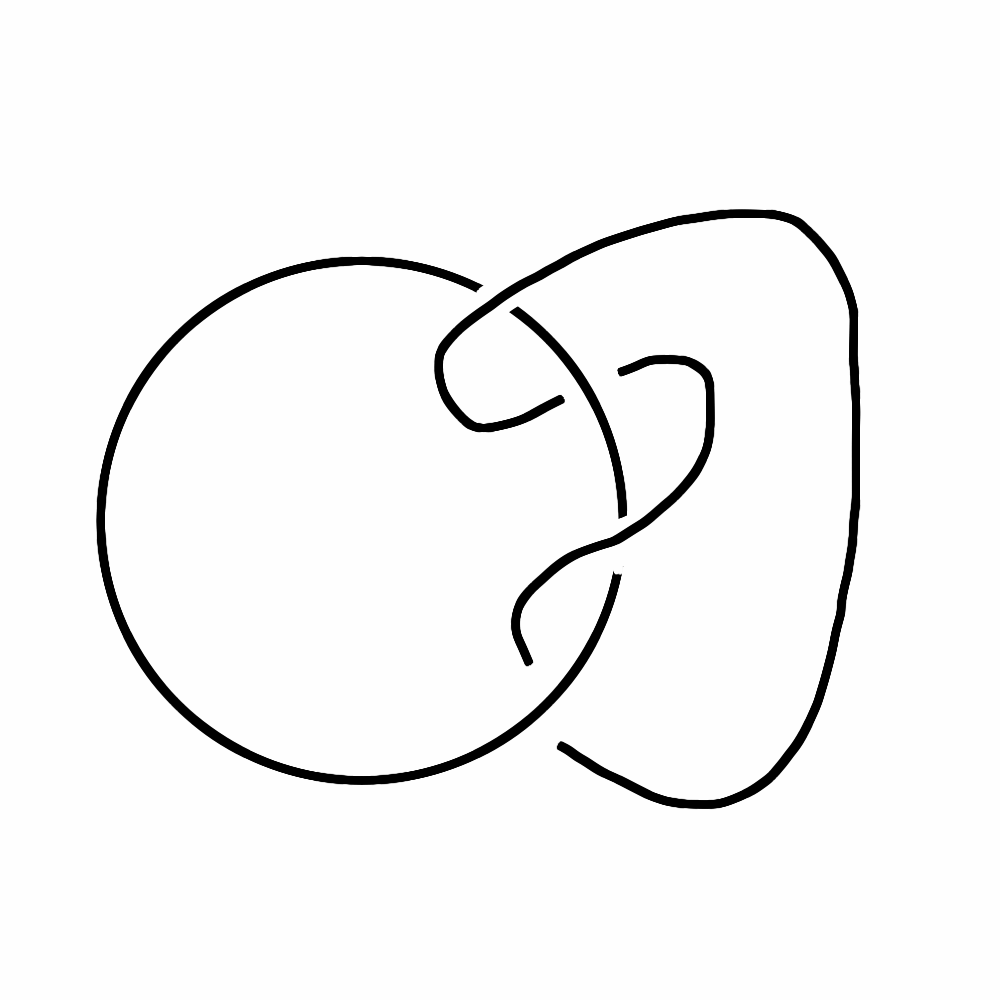
\includegraphics[width=\textwidth]{knotpics/lno2.png}
        \caption{Link A}
    \end{subfigure}
    \hspace{1cm}
    \begin{subfigure}{.3\textwidth}
        \centering         
        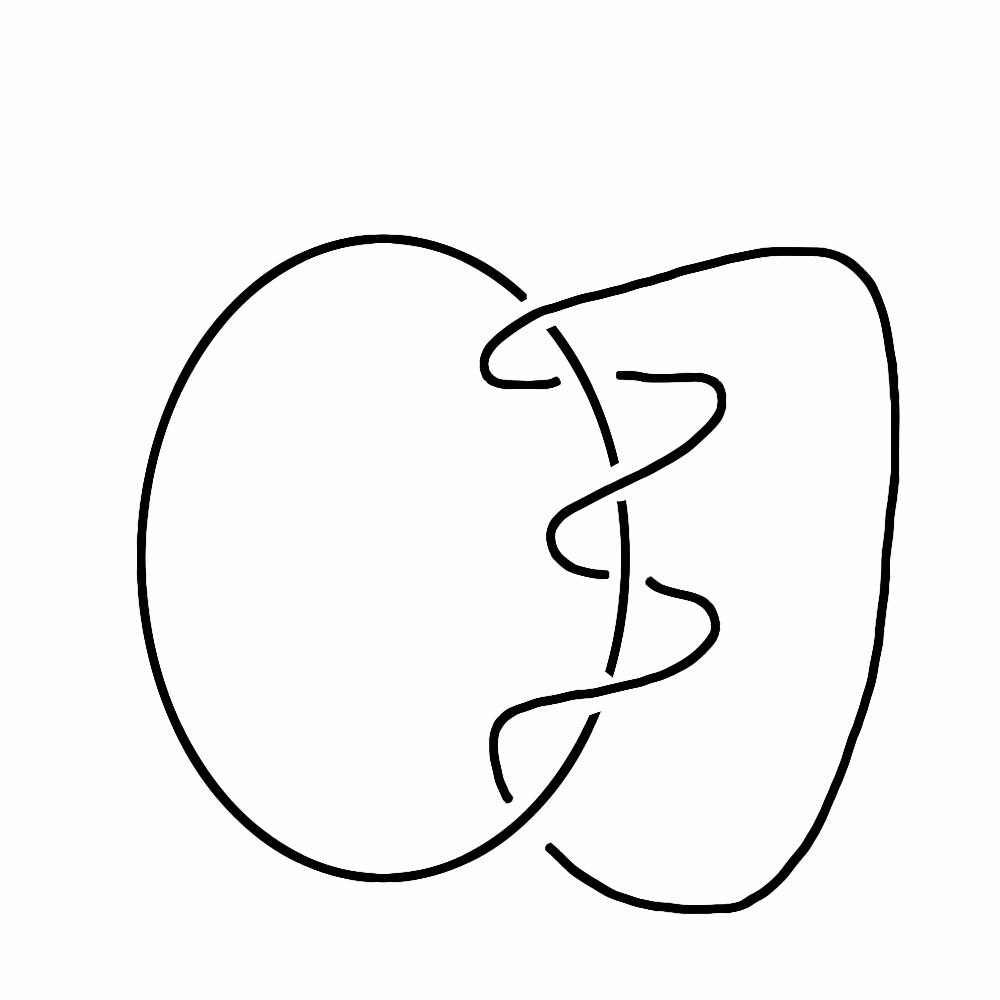
\includegraphics[width=\textwidth]{knotpics/lno3.png}
        \caption{Link B}
    \end{subfigure}
    \caption{Two Links \textbf{not} distinguished by our current invariants.}
\end{figure}


Both of these links have two components, and neither is tricolorable.
They certainly \emph{seem} different, though.
Somehow, Link B looks ``more linked'' than Link A.
Our goal for this reading is to learn a new invariant that will distinguish between these two links.

\section*{Linking Number}

\subsection*{Choosing Orientation}

An \emph{orientation} on a knot is a choice of direction of travel along the knot.
Each knot has two of these. 
(If one is forward, then the other is reverse.)
We can indicate an orientation on a knot by drawing an arrow.

\begin{figure}[h]
    \centering
    \begin{subfigure}{.3\textwidth}
        \centering
        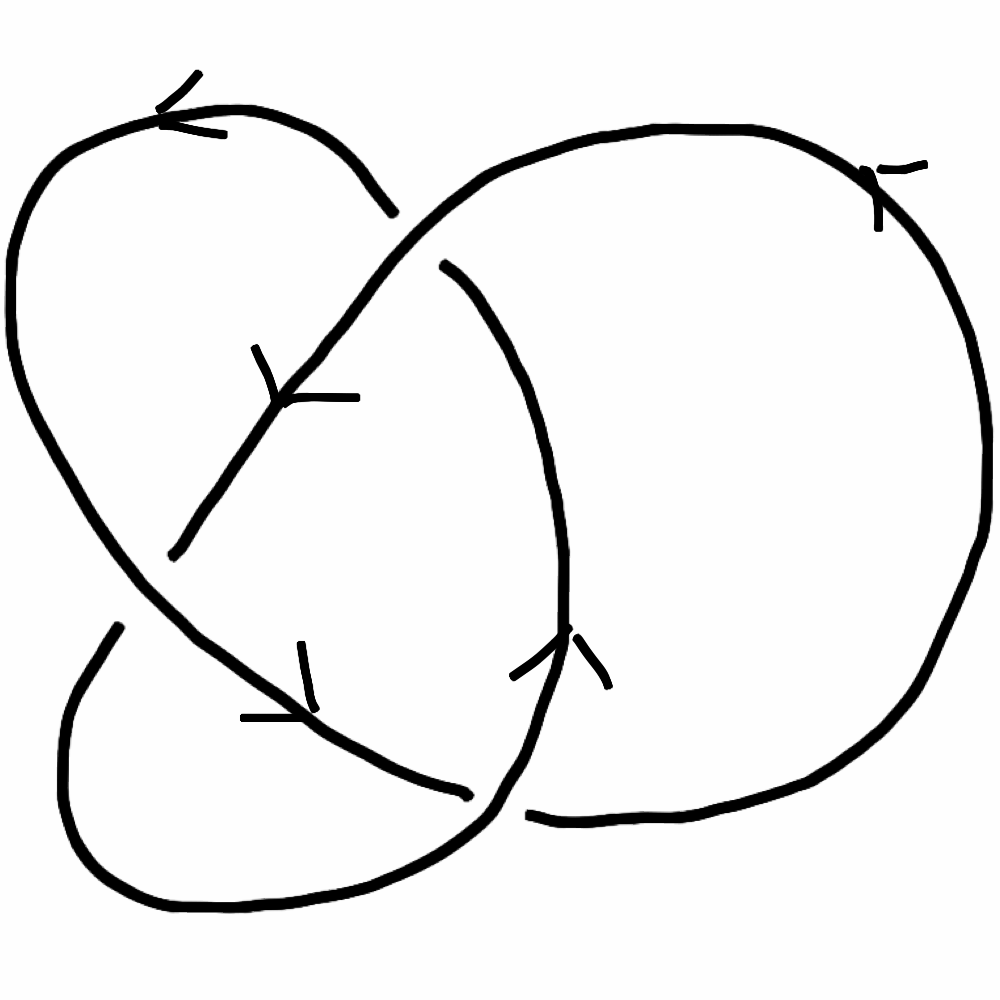
\includegraphics[width=\textwidth]{knotpics/trefoil-forward.png}
    \end{subfigure}
    \hspace{1cm}
    \begin{subfigure}{.3\textwidth}
        \centering         
        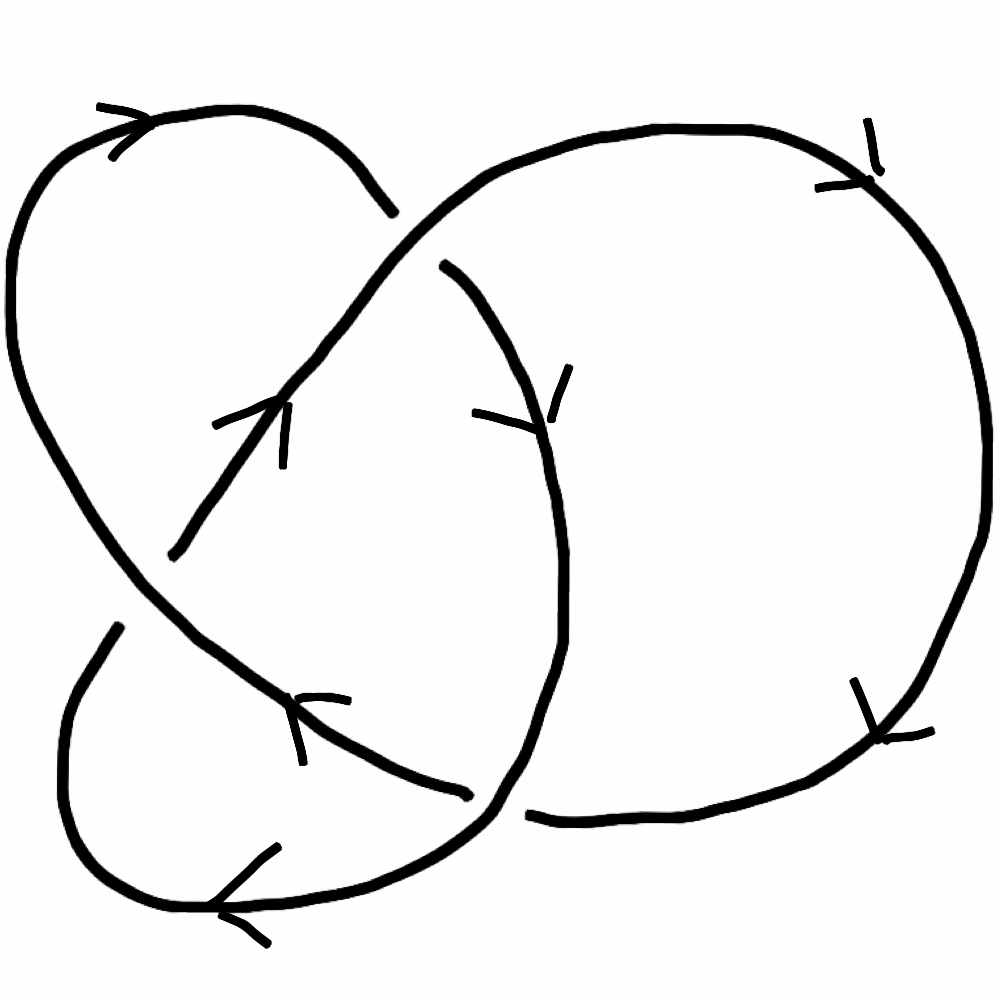
\includegraphics[width=\textwidth]{knotpics/trefoil-reverse.png}
    \end{subfigure}
    \caption{Two orientations on the trefoil knot.}
\end{figure}

For a link, each component is a knot. 
An \emph{orientation} on a link is a choice of orientation for each component of a knot.
For example, here are two orientations on a three component link.

\begin{figure}[h]
    \centering
    \begin{subfigure}{.3\textwidth}
        \centering
        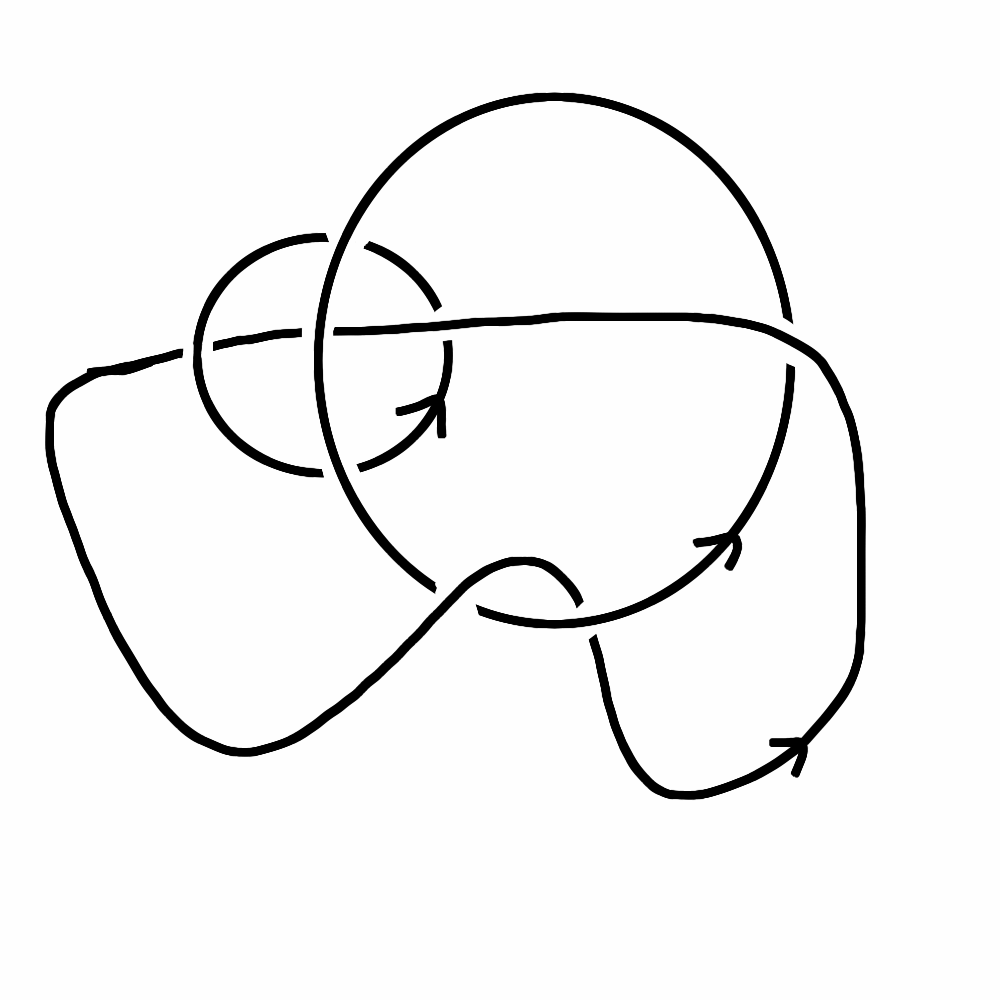
\includegraphics[width=\textwidth]{knotpics/threelinka.png}
    \end{subfigure}
    \hspace{1cm}
    \begin{subfigure}{.3\textwidth}
        \centering         
        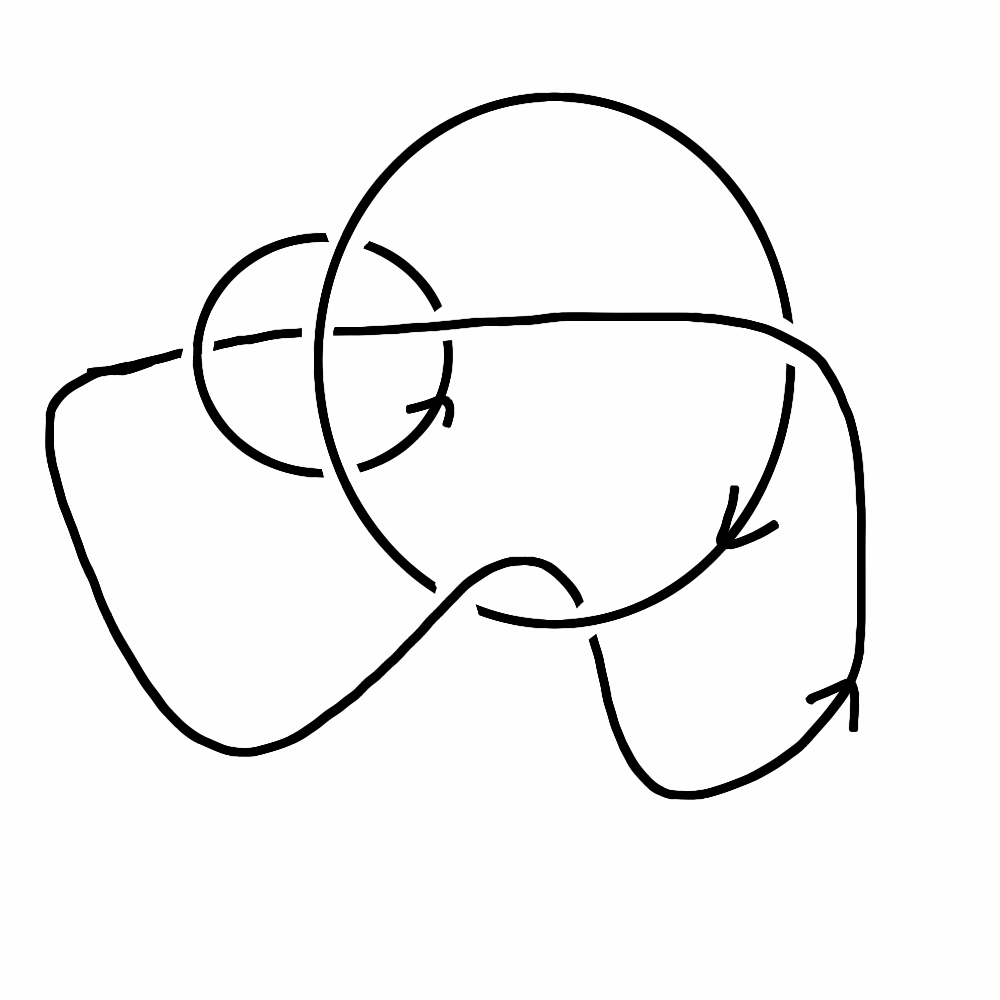
\includegraphics[width=\textwidth]{knotpics/threelinkb.png}
    \end{subfigure}
    \caption{Two orientations on a three component link, $L$.}
\end{figure}

\begin{exercise}
The link $L$ given above has three components, so it has 8 orientations.
Draw the other six.
\end{exercise}

\clearpage

\subsection*{Classifying crossings}

After choosing an orientation, crossings will look like one of these two:

\begin{figure}[h]
    \centering
    \begin{subfigure}{.3\textwidth}
        \centering
        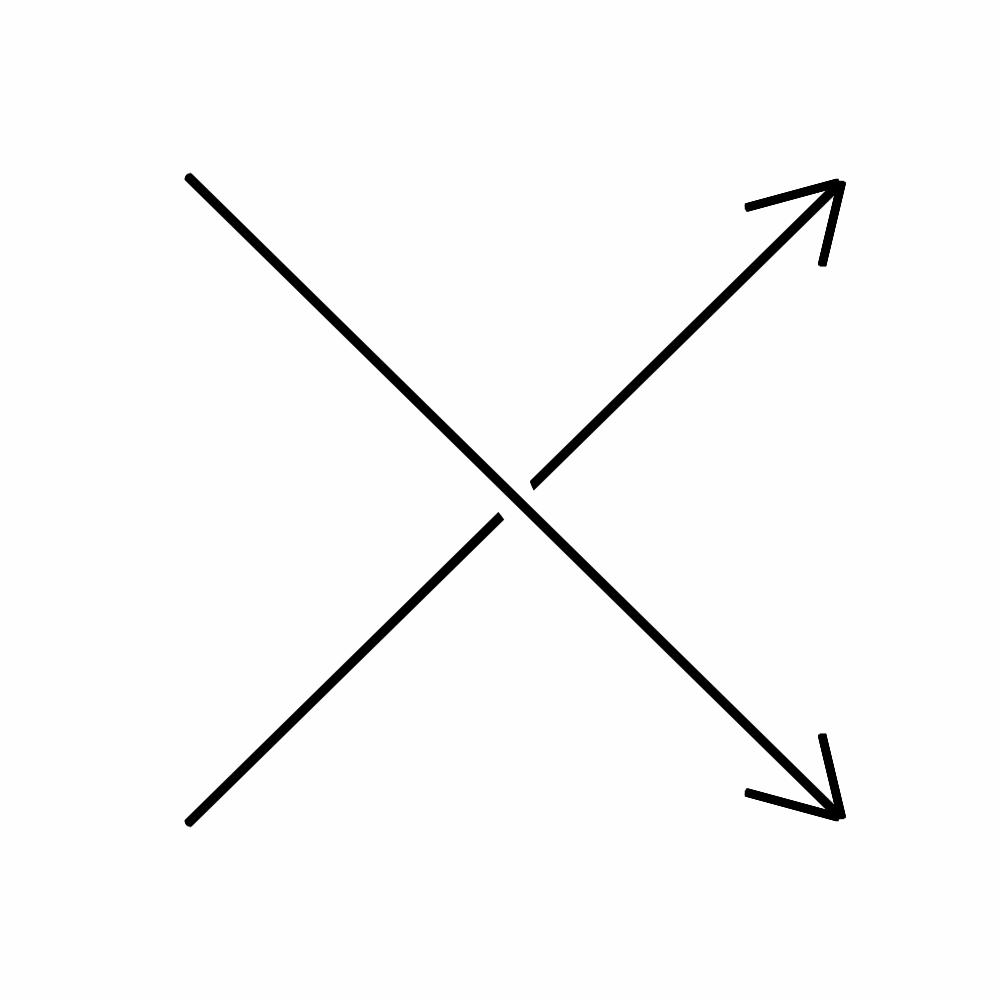
\includegraphics[width=\textwidth]{knotpics/poscross.png}
        \caption{$+1$}
    \end{subfigure}
    \hspace{1cm}
    \begin{subfigure}{.3\textwidth}
        \centering         
        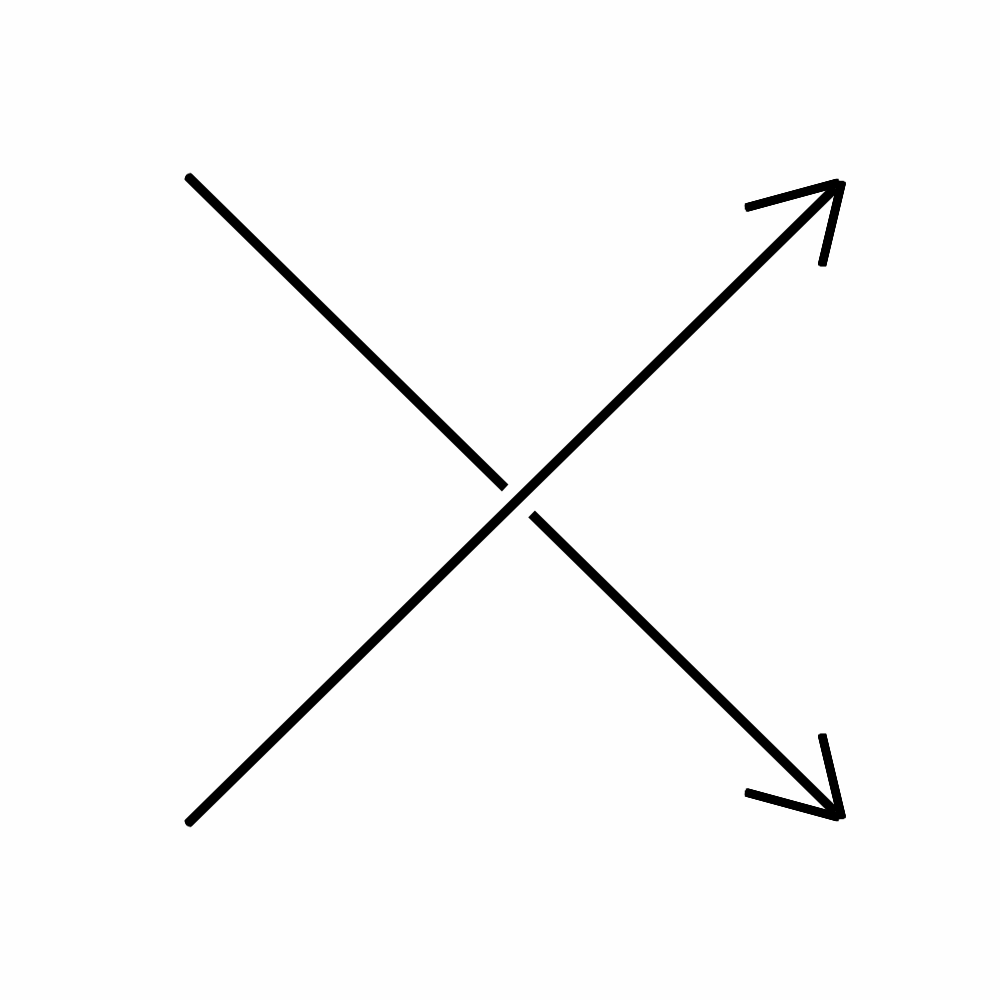
\includegraphics[width=\textwidth]{knotpics/negcross.png}
        \caption{$-1$}
    \end{subfigure}
    \caption{The two types of crossing.}
\end{figure}

Now we assign each crossing a $+1$ or a $-1$.
The key to telling the difference is in which way we rotate the understrand to line up the arrows.
If you rotate the understrand clockwise to line up the arrows, the crossing is a $+1$.
If you rotate the understrand counter-clockwise to line up the arrows, the crossing is a $-1$.

\subsection*{Linking Number of Two Components}

The linking number is a number associated to a pair of components in a link. 
So if the link has three or more components, it will have \underline{several} linking numbers, depending on which choice of components is made.

Consider our example from above.
To keep things straight, let's color the three components differently.
This will allow us to tell them apart.
We will use the coloring and the orientation shown in this planar projection.

\begin{figure}[h]
    \centering
    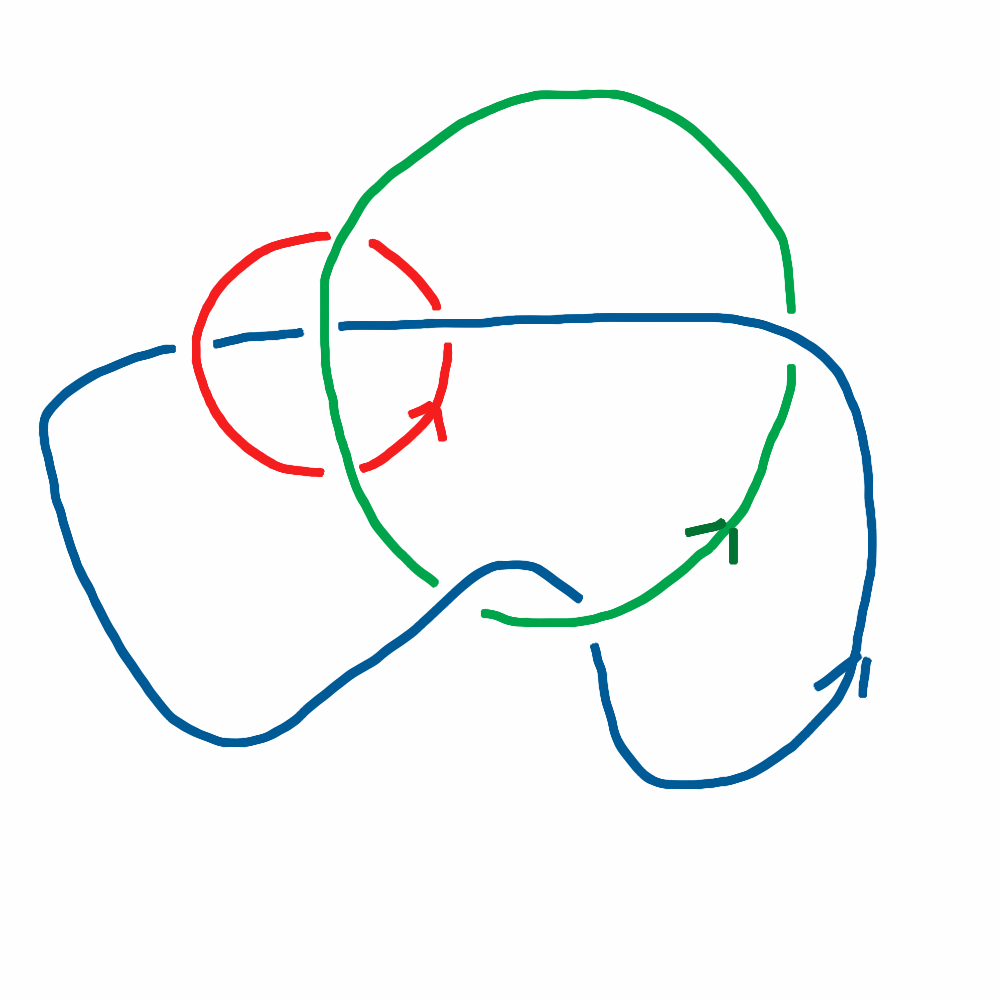
\includegraphics[width=.35\textwidth]{knotpics/mainex.png}
    \caption{The Main Example}
\end{figure}


\begin{wrapfigure}{L}{.3\textwidth}
    \centering
    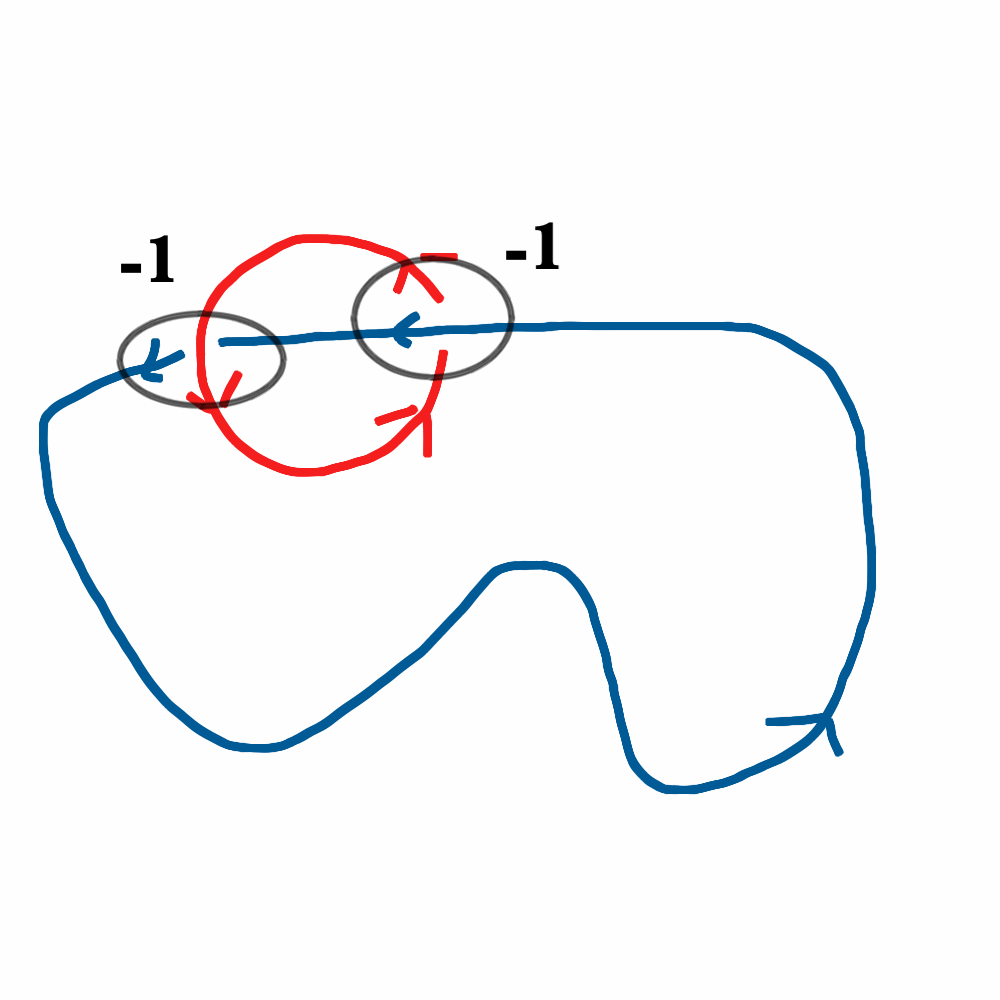
\includegraphics[width=.3\textwidth]{knotpics/rb.png}
    \caption{Just the red and blue components.}
    \vspace{-60pt}
\end{wrapfigure}
We start with the linking number of the red and blue components.
\begin{description}
\item[Step 1] Isolate just the two oriented components of interest, and ignore the others.

\item[Step 2] Check each crossing \textbf{that involves both components} and label them $+1$ or $-1$ by the rule above. Do not consider any crossings where one component crosses itself.
\item[Step 3] Do a numerical computation: add the numbers on the crossings, divide the result by 2, then take the absolute value.
\[ 
\mathrm{link}(\text{red}, \text{blue}) = \left| \dfrac{(-1)+(-1)}{2}\right| = 1.
\]
\end{description}


\begin{wrapfigure}{R}{.3\textwidth}
    \centering
    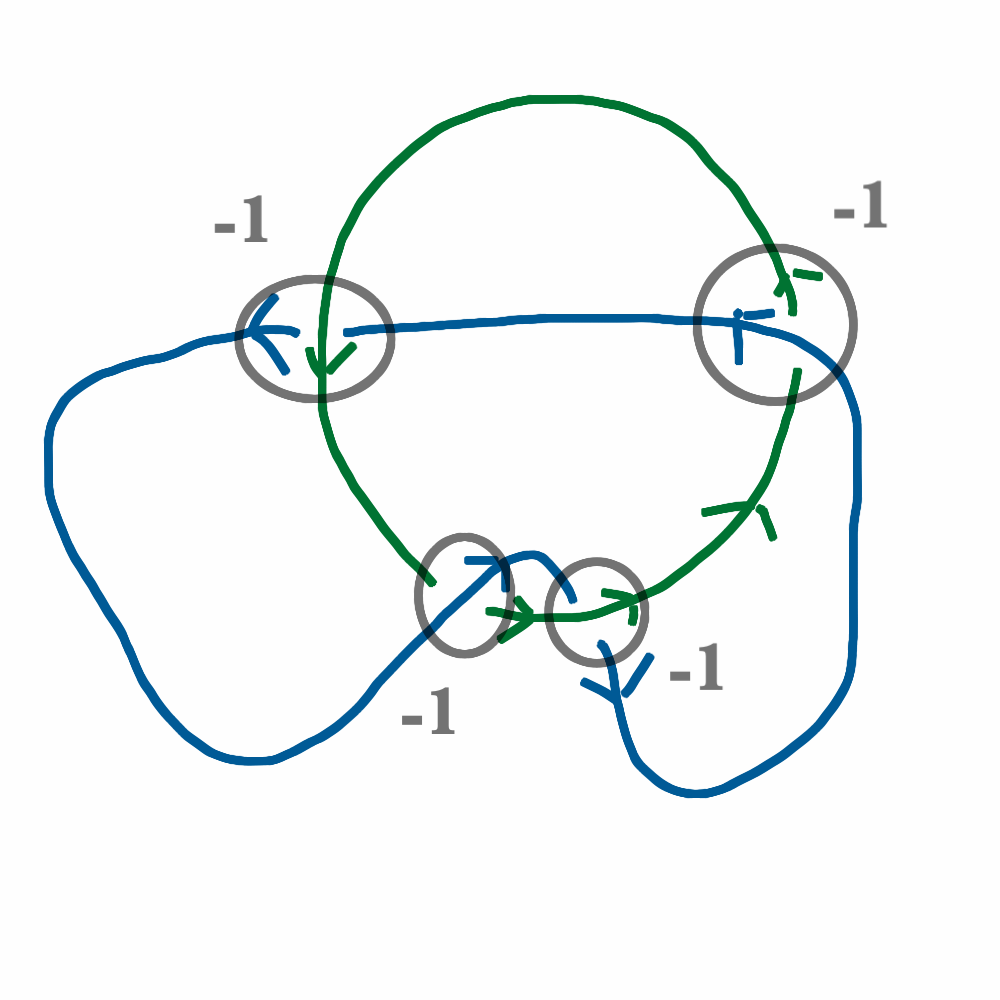
\includegraphics[width=.3\textwidth]{knotpics/bg.png}
    \caption{Just the blue and green components.}
\end{wrapfigure}

\vspace{1in}

Just to be clear, we check the same thing for the blue and green components.
We isolate the blue and green component knots, label the crossings between the two components, and then compute the linking number following the rule.
\[
\mathrm{link}(\text{blue},\text{green}) = \left| \dfrac{ (-1)+(-1)+(-1)+(-1)}{2}\right| = 2
\]


\begin{exercise}
Verify that $\mathrm{link}(\text{red},\text{green}) = 0$.
\end{exercise}


It is worth noting that the absolute value plays a simple role here.
If we change the orientation of one of the two components, all the signs will get changed!
The absolute value makes sure that we do not notice this choice in our computation.
All that matters is how twisted together the components are, not what choice of orientation we made.

\begin{challenge}
Check the claim about orientation: 
Change the direction of the blue component and redo the last two computations to see what happens.
\end{challenge}


\clearpage

Now it is time to get some practice.

\begin{exercise} 
The three links below each have two components, so each only has one linking number.
Compute these numbers.
\end{exercise}

\begin{figure}[h]
    \centering
    \begin{subfigure}{.3\textwidth}
        \centering
        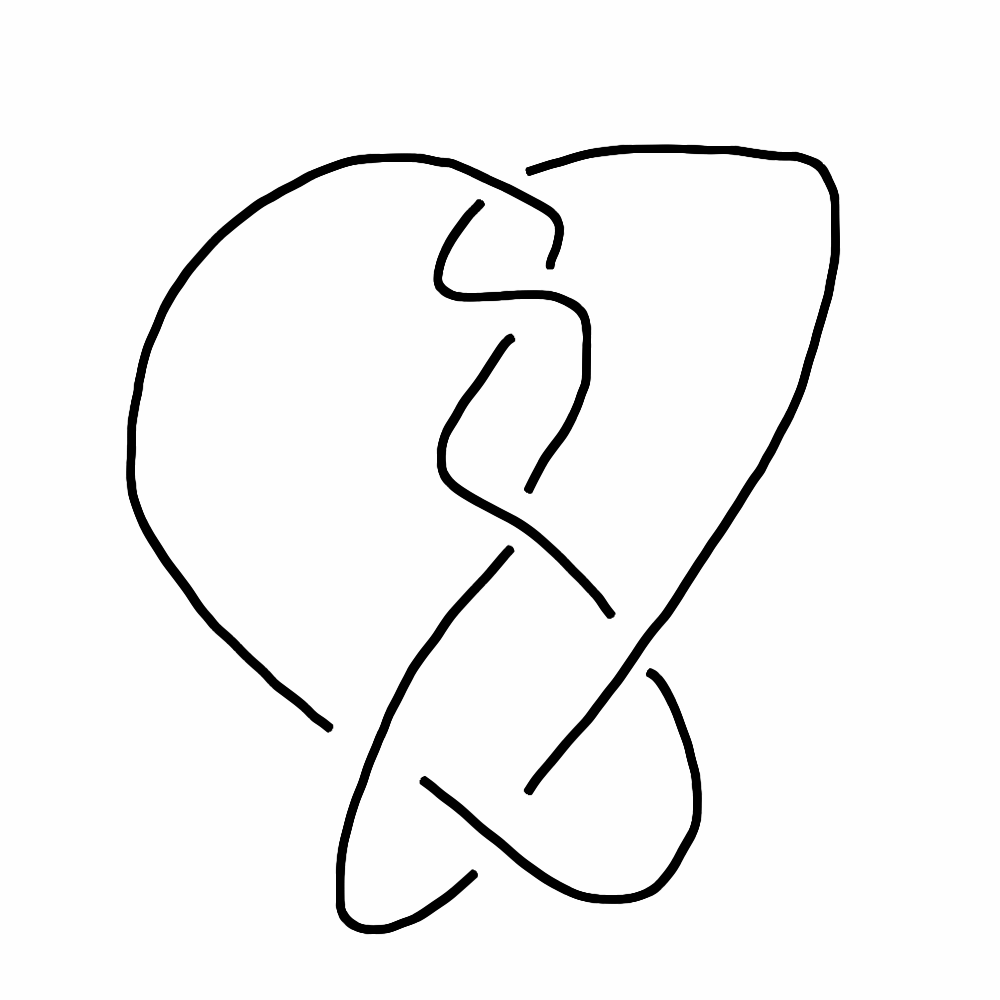
\includegraphics[width=\textwidth]{knotpics/ex1.png}
    \end{subfigure}
    \quad
    \begin{subfigure}{.3\textwidth}
        \centering
        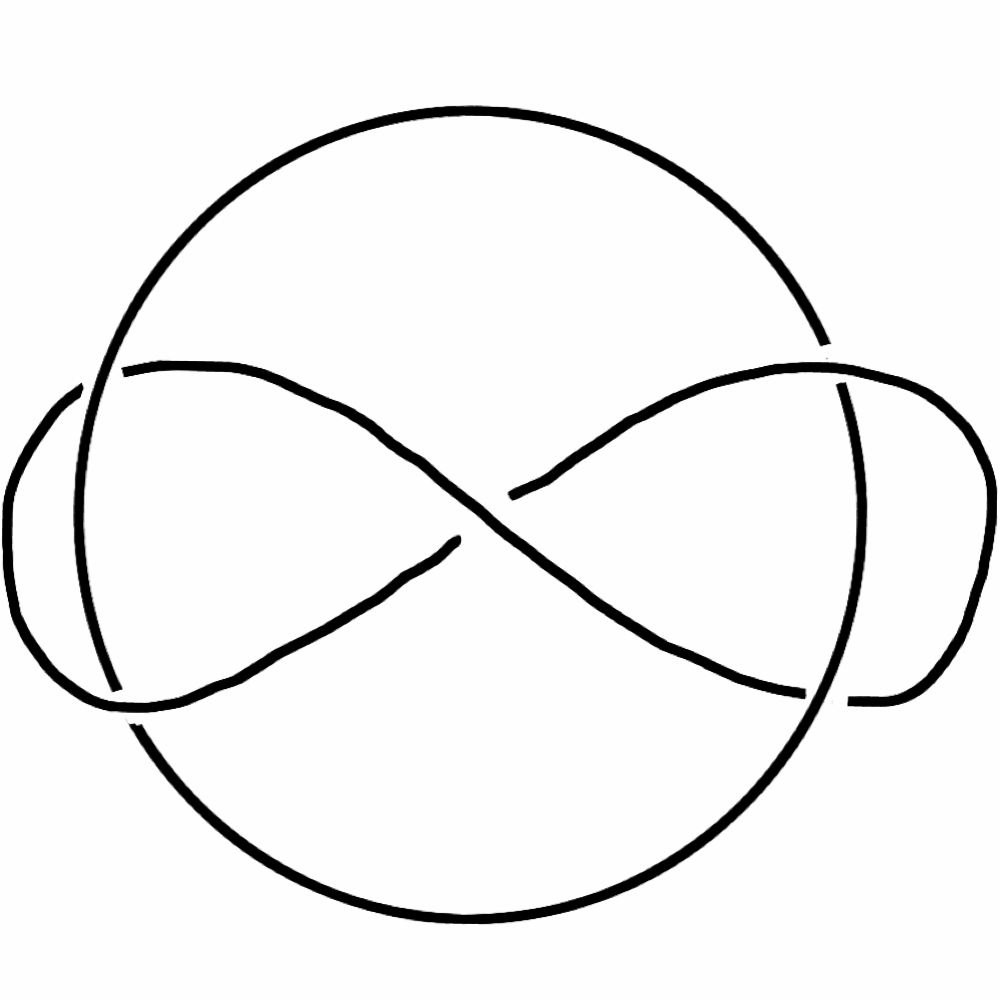
\includegraphics[width=\textwidth]{knotpics/ex2.png}
    \end{subfigure}
    \quad
    \begin{subfigure}{.3\textwidth}
        \centering
        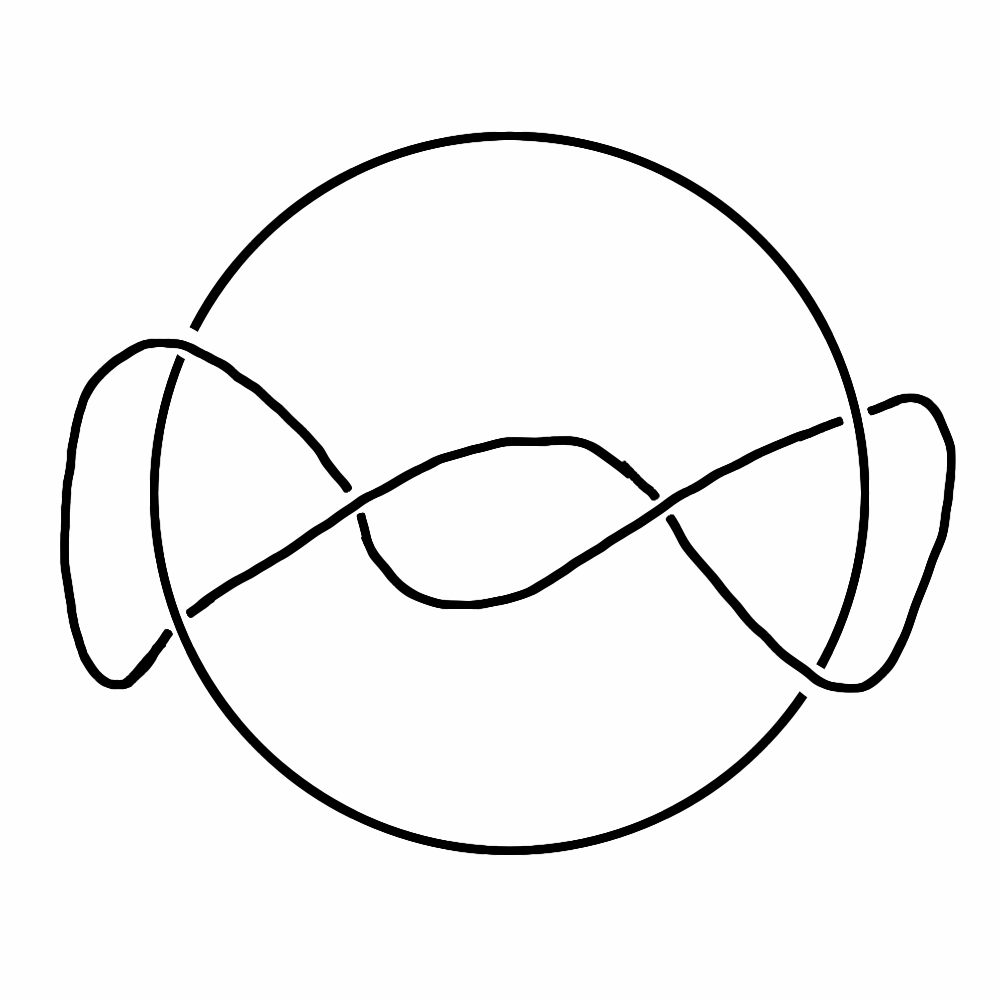
\includegraphics[width=\textwidth]{knotpics/ex3.png}
    \end{subfigure}
    \caption{Three links, each with two components.}
\end{figure}
    
\begin{exercise}
The link below has three components.
Compute the linking number of each pair.
\end{exercise}

\begin{figure}[h]
    \centering
    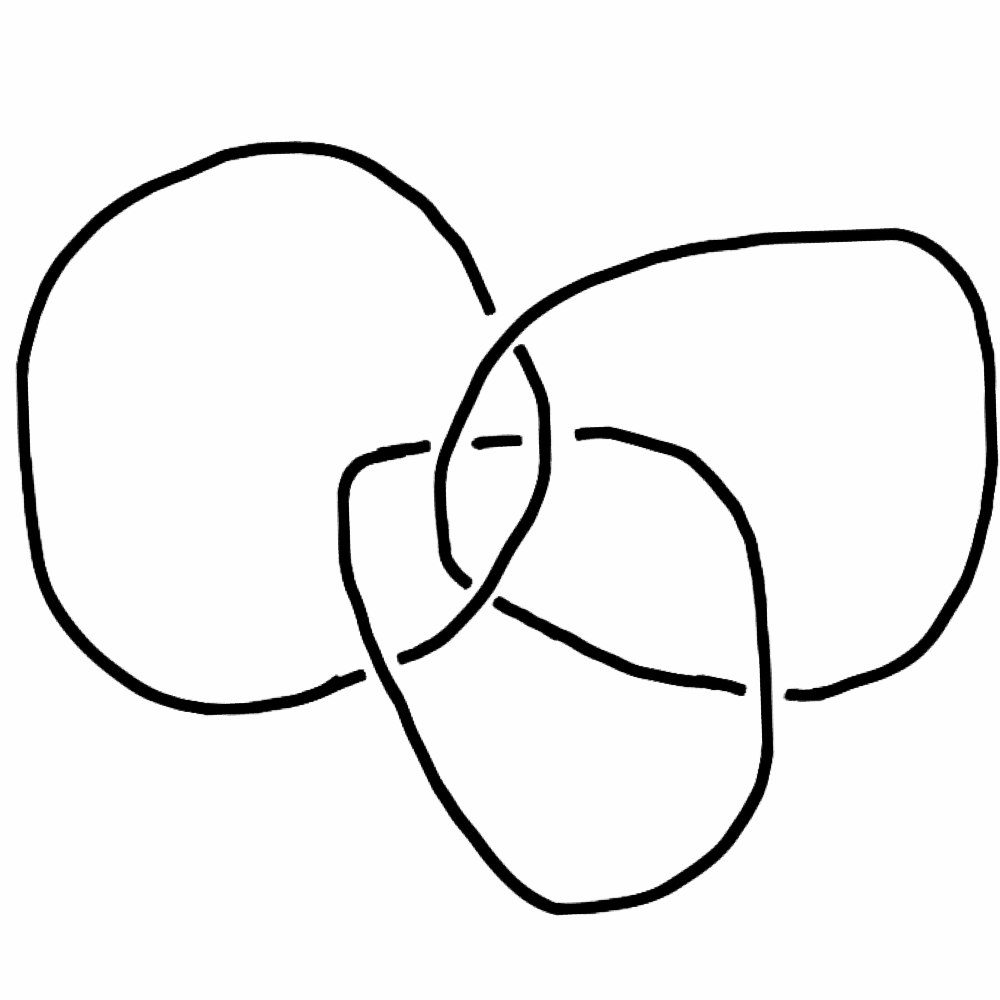
\includegraphics[width=.5\textwidth]{knotpics/hitchmantriple.png}
    \caption{A Link of 3 components.}
\end{figure}

\clearpage

\subsection*{The Linking Numbers are Invariants}

The linking number of two components is an invariant of links under ambient isotopy.
That is, if we change one link into another by an ambient isotopy, none of the linking numbers will change.
The way to verify this is to check what happens when you use a Reidemeister move!

\begin{challenge}
For each type of Reidemeister move diagram, check that linking number won't change.
\end{challenge}

\subsection*{A Challenge Question}

In the examples above, we have seen linking numbers for two components that take the values $0, 1, 2$, \emph{etc.}
Suppose we want to generate other values.
Is that possible?
What about $7$? $13$? $44$?

\begin{challenge}
What linking numbers are possible?
How can you find a family of two component links which realize these numbers?
(Hint: Go back to the examples in Figure 1.)
\end{challenge}


\begin{thebibliography}{9}
\bibitem{Adams}
	Colin C. Adams,
	\emph{The Knot Book},
	American Mathematical Society, 
	2004.	
\end{thebibliography}

\end{document}
%sagemathcloud={"zoom_width":100}